\chapter{Инструмент фаззинг-тестирования AFL++} \label{ch3}

% не рекомендуется использовать отдельную section <<введение>> после лета 2020 года
%\section{Введение} \label{ch3:intro}

\textit{AFL++} - это улучшенная версия популярного инструмента фаззинга AFL (American Fuzzy Lop), разработанная сообществом для повышения его эффективности и функциональности. \textit{AFL} — это ориентированный на поиск ошибок инструмент анализа ПО, который использует обширный список типов инструментации кода для получения информации о покрытии и множество генетических алгоритмов мутации для автоматического обнаружения различных тестовых примеров, которые вызывают новые внутренние состояния в бинарном коде ПО. Фаззер AFL поддерживает инструментацию, реализующуюся на этапе компиляции из исходного кода с помощью оберток afl-gcc/afl-g++. afl-gcc/afl-g++ подменяет вызываемую команду на обертку, переписывающую ассемблерный код, сгенерированный компилятором. Для фаззинга уже скомпилированных бинарных файлов используется qemu mode — это патч к QEMU, эмулирующий запуск одного процесса и реализующий требуемую для анализа инструментацию кода [8].
\par
AFL является одним из самых известных фаззеров серого ящика, он поддерживает фаззинг программ, написанных на C, C++ и Objective C, скомпилированных с помощью и GCC, и CLang, но его часто расширяют и портируют.
\par
AFL требует от пользователя предоставить пример команды, запускающей тестируемое приложение, и хотя бы один небольшой пример входных данных. Входные данные могут быть переданы в тестируемую программу либо через стандартный ввод, либо в виде входного файла, указанного в командной строке процесса. Чтобы максимизировать производительность фаззинга, American fuzzy lop ожидает, что тестируемая программа будет скомпилирована с помощью служебной программы, которая оснащает (инструментирует) код вспомогательными функциями, которые отслеживают поток управления.

\section{Инструментирование} \label{ch3:sec1}
Инструментирование – это процесс внедрения дополнительного кода или инструкций в исходный код программы с целью сбора информации о её выполнении.
Это позволяет фаззеру:
\begin{itemize}
	\item Отслеживать, какие части кода выполняются (покрытие кода).
	\item Определять, какие новые ветви кода (пути выполнения) были исследованы благодаря новым или мутированным входным данным.
	\item Собирать статистику о выполнении для последующего анализа.
\end{itemize}
\par
AFL представляет собой фаззер серого ящика , то есть он внедряет инструменты для измерения покрытия кода в целевую программу во время компиляции и использует метрику покрытия для управления генерацией новых входных данных.
В случаях, когда это невозможно, также поддерживается тестирование «черного ящика» [2].

\section{Измерение покрытия} \label{ch3:sec2}
AFL подсчитывает количество раз, которое данное выполнение целевой программы проходит через каждое ребро в графе управления потоком целевой программы; Ребро в графе управления потоком (control-flow graph, CFG) программы представляет собой переход между двумя узлами (которые представляют собой отдельные блоки инструкций). 
\par
AFL поддерживает глобальный набор пар (словарь) которые были произведены любым выполнением до этого момента. Входные данные считаются "интересными" и добавляются в очередь, если они производят пару, которой ещё нет в словаре.
\par
Инструментарий, внедряемый в скомпилированные программы, фиксирует покрытие ветвей (рёбер), а также подсчеты срабатываний условных переходов. Точки ветвления в контексте программирования — это места в коде, где происходит условный переход, который может изменить путь выполнения программы. Например, это могут быть операторы if, switch, циклы, или даже вызовы функций — все, что может привести к изменению последовательности исполняемых инструкций [4]. 
\par
Код, вставляемый в точках ветвления, по существу включает следующее:

\begin{algorithm}
	\SetAlgoLined 
	\DontPrintSemicolon 
	
	\BlankLine
	$cur\_location \gets \langle COMPILE\_TIME\_RANDOM \rangle$\;
	\BlankLine
	\ForEach{$prev\_location$}{
		$shared\_mem[cur\_location \oplus prev\_location]++$\;
		$prev\_location \gets cur\_location \gg 1$\;
	}
	\caption{Код, измеряющий покрытие, внедряемый в точки ветвления}
	\label{alg:AlgoFDSCALING}
\end{algorithm}

\textbf{cur\textunderscore location}:
Это переменная, которая используется как идентификатор текущего места в коде, где выполняется операция инструментирования. Значение cur\textunderscore location генерируется случайно на этапе компиляции и уникально для каждой точки ветвления. Оно используется для того, чтобы отслеживать, была ли достигнута эта точка ветвления при выполнении программы.

\textbf{shared\textunderscore mem}:
shared\textunderscore mem — это массив, который используется как словарь покрытия для отслеживания, какие точки ветвления (и переходы между ними) были выполнены во время исполнения программы. Ключем является xor (prev\textunderscore location, cur\textunderscore location), а значением счетчик попаданий для данного кортежа (перехода). Каждый раз, когда исполнение программы проходит через этот переход, счетчик увеличивается

\textbf{prev\textunderscore location}:
помогает отслеживать предыдущее состояние исполнения программы и выявлять изменения в путях исполнения при каждой новой итерации фаззинга.

\par
Размер словаря выбран таким образом, чтобы коллизии возникали редко для почти всех предполагаемых целей. Коллизии могут возникать, например, когда несколько различных входных данных приводят к одной и той же точке ветвления (branch) в программе или к одному и тому же состоянию программы.
На \firef{fig:coverage-measuring-ch3} представлена зависимость количества коллизий от количества ветвлений.

\begin{figure}[ht] 
	\center
	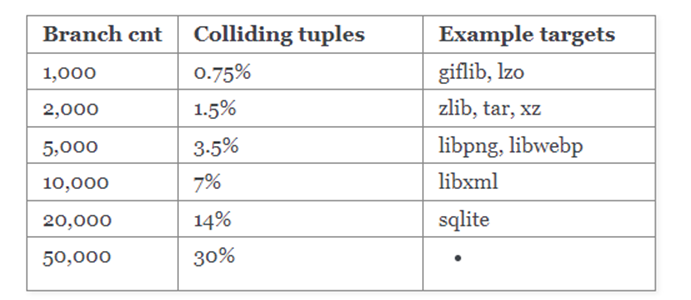
\includegraphics [scale=1] {my_folder/images/coverage_measuring}
	\caption{Распределение количества коллизий кортежей при различном количестве ветвлений для разных целей фаззинга} 
	\label{fig:coverage-measuring-ch3}  
\end{figure}

В то же время размер словаря достаточно мал, чтобы анализ словаря занимал всего лишь несколько микросекунд и чтобы словарь легко помещался в кэш второго уровня (L2 cache) [4].
\par
Такая форма покрытия предоставляет значительно более глубокое представление о пути выполнения программы, в частности, она тривиально различает следующие трассы исполнения:
\par
A -> B -> C -> D -> E (кортежи: AB, BC, CD, DE) и 
\par
A -> B -> D -> C -> E (кортежи: AB, BD, DC, CE)

\section{Обнаружение нового поведения} \label{ch3:sec3}
Фаззер поддерживает глобальный словарь кортежей, замеченных в предыдущих исполнениях, эти данные можно быстро сравнить с отдельными трассами и обновить.
\par
Когда измененный вход генерирует трассировку выполнения, которая содержит новые кортежи, соответствующий входной файл будет сохранен и направлен для дополнительной обработки позже. Входы, которые не инициируют новые переходы состояний локального масштаба во время отслеживания выполнения (например, не генерируют новые кортежи), будут отброшены, даже если их общий поток управления уникален.
\par
В дополнение к обнаружению новых кортежей фаззер также учитывает приблизительное количество кортежей. Они разделены на несколько частей:
1, 2, 3, 4-7, 8-15, 16-31, 32-127, 128+.
\par
Эта упрощенная классификация помогает фаззеру быстро определить "интересные" изменения в потоке управления программы без необходимости в точном подсчете каждого выполнения. Вместо того, чтобы отслеживать каждое выполнение отдельно, фаззер смотрит на общую картину и обнаруживает изменения, которые выходят за пределы ожидаемых или типичных паттернов выполнения программы.
\section{Изменение очереди ввода} \label{ch3:sec4}
Тестовые случаи мутации, которые генерируют новые переходы состояний в программе, добавляются во входную очередь и служат отправной точкой для будущих циклов фаззинга. Они дополняют, но не могут автоматически заменить существующие открытия.
В отличие от более жадных генетических алгоритмов, этот подход позволяет инструменту постепенно исследовать различные непересекающиеся и, возможно, взаимно несовместимые функции базового формата данных, как показано на \firef{fig:test-generation-ch3} [4].

На \firef{fig:coverage-measuring-ch3} представлена зависимость количества коллизий от количества ветвлений.

\begin{figure}[ht] 
	\center
	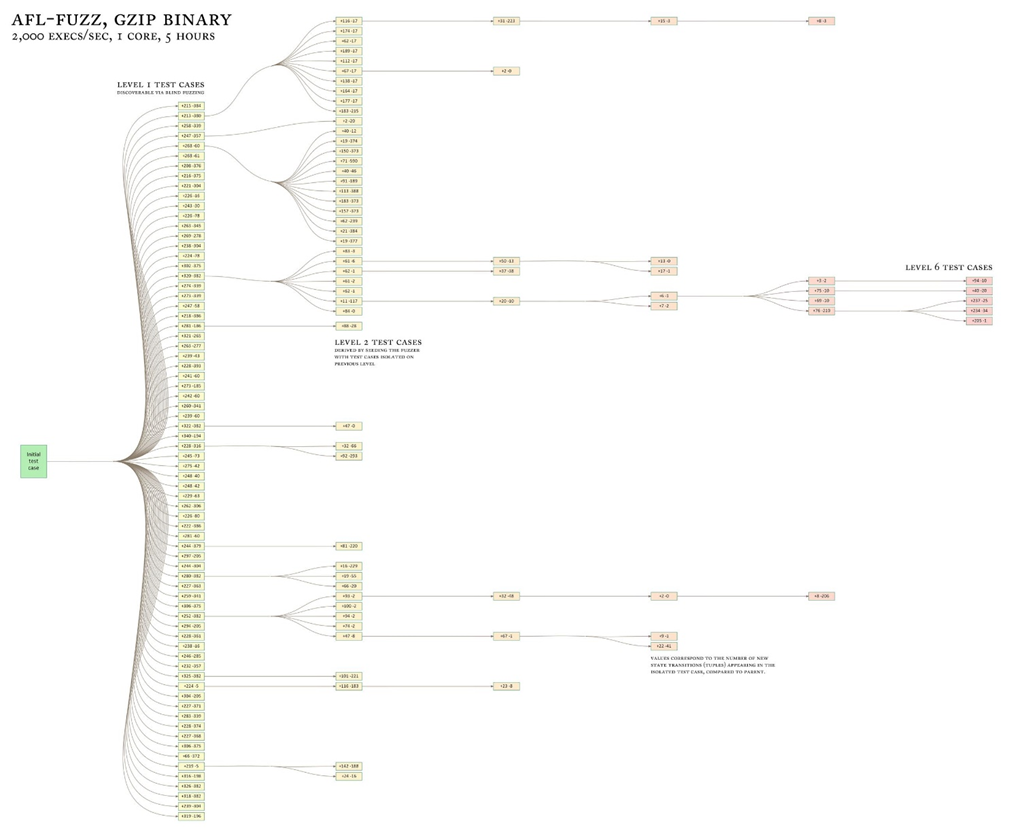
\includegraphics [scale=1] {my_folder/images/test_gen}
	\caption{Визуализация дерева тестирования AFL-Fuzz} 
	\label{fig:test-generation-ch3}  
\end{figure}
\par
В общем, AFL поддерживает очередь, и каждый раз, когда файл берется из этой очереди, в нее вносится множество мутаций, и проверяется, не обнаружит ли новые пути после операции.

\section{Отбраковка корпуса} \label{ch3:sec5}
Корпус (corpus) - это коллекция тестовых данных или файлов, которые используются для проведения тестирования программы или системы. Корпус включает в себя как исходные тестовые данные, так и те, которые были сгенерированы или изменены в ходе тестирования.
\par
Подход к пошаговому исследованию состояний, описанный выше, означает, что некоторые тестовые случаи, синтезированные позднее, могут иметь покрытие ветвей, которое является строгим надмножеством покрытия, предоставленного их предками. Чтобы оптимизировать процесс фаззинга, AFL периодически переоценивает очередь, используя быстрый алгоритм, который выбирает меньшее подмножество тестовых примеров, которые по-прежнему охватывают каждый кортеж, виденный на данный момент, и характеристики которых делают их особенно благоприятными для инструмента.
\par 
Сгенерированный корпус "предпочтительных" записей обычно в 5-10 раз меньше, чем исходный набор данных. Непредпочтительные записи не удаляются, но они пропускаются с различными вероятностями при обнаружении в очереди:

\begin{itemize}
	\item Если в очереди есть новые, еще не прошедшие фаззинг, предпочтительные записи, 99\% непредпочтительных записей будут пропущены, чтобы достичь предпочтительных.
	\item Если нет новых предпочтительных записей:
	\begin{itemize}
		\item Если текущая непредпочтительная запись уже прошла через фаззинг, она будет пропущена в 95\% случаев.
		\item Если она еще не прошла ни одного фаззинга, вероятность пропуска уменьшается до 75\%.
	\end{itemize}
\end{itemize}

\par
Это обеспечивает разумный баланс между скоростью цикла очереди и разнообразием тестовых случаев [4].

\section{Стратегии фаззинга, предоставляемые AFL++} \label{ch3:sec6}

Для генерации новых входных данных AFL применяет различные мутации к существующим данным. Эти мутации в основном нечувствительны к формату входных данных целевой программы; они обычно обрабатывают входные данные как простой массив бинарных данных.

Сначала AFL применяет детерминированную последовательность мутаций к каждому входному файлу. Они применяются в различных местах входных данных и включают:
\begin{itemize}
	\item Инвертирование (т.е. отрицание или инвертирование) от 1 до 32 бит.
	\item Инкрементирование и декрементирование 8-, 16- и 32-битных целых чисел в кодировках как little-endian, так и big-endian.
	\item Перезапись частей входных данных "примерно двумя десятками 'интересных' значений", включая ноль, максимальные и минимальные знаковые и беззнаковые целые различной ширины, также в кодировках little- и big-endian.
	\item Замена частей входных данных данными, взятыми из "словаря" пользовательских или автоматически обнаруженных токенов (например, магические байты или ключевые слова в текстовом формате).
\end{itemize}

После применения всех доступных детерминированных мутаций AFL переходит к стадии "havoc", на которой подряд применяются от 2 до 128 мутаций. Эти мутации включают описанные выше детерминированные мутации, а также:
\begin{itemize}
	\item Перезапись байтов случайными значениями.
	\item Операции над многобайтовыми "блоками":
	\begin{itemize}
		\item Удаление блоков.
		\item Дублирование блоков.
		\item Установка каждого байта в блоке в одно значение.
	\end{itemize}
\end{itemize}

Если AFL проходит через всю очередь, не генерируя ни одного входа, который достигает нового покрытия кода, он начинает "склеивание". Склеивание берет два входа из очереди, обрезает их в произвольных позициях, соединяет их вместе и применяет к результату стадию "havoc"  [2].

\subsection{Стратегия фаззинга: Bit flips} \label{ch2:bit-flips}
Первая и наиболее элементарная стратегия, используемая afl включает в себя выполнение последовательных, упорядоченных переворотов битов. Переход всегда составляет один бит; количество бит, переворачиваемых подряд, варьируется от одного до четырех. Для большого и разнообразного массива входных файлов наблюдаемые результаты следующие:

\begin{itemize}
	\item Переключение одного бита: ~ 70 новых путей на миллион сгенерированных входных данных
	\item Переключение двух битов подряд: ~ 20 дополнительных путей на миллион сгенерированных входных данных
	\item Переключение четырех битов подряд: ~ 10 дополнительных путей на миллион входных данных [5].
\end{itemize}

\begin{figure}[ht]
	\begin{lstlisting}[language=C]
		#define FLIP_BIT(_ar, _b) do { 
			u8 *_arf = (u8 *)(_ar);      
			u32 _bf = (_b);              
			_arf[(_bf) >> 3] ^= (128 >> ((_bf) & 7)); 
		} while (0)
	\end{lstlisting}
	\caption{Реализация алгоритма bit flip в AFL++}\label{fig:flip-bit}
\end{figure}

Этот макрос переворачивает конкретный бит в массиве. Он использует \textunderscore ar для указания на массив, а \textunderscore b для указания на бит, который нужно перевернуть. Переворот осуществляется путём применения операции XOR к соответствующему байту и биту в этом байте.

\subsection{Стратегия фаззинга: Byte flips} \label{ch2:byte-flips}
Естественное продолжение подхода пошагового переворота битов, этот метод основан на битовых переворотах шириной 8, 16 или 32 бита с постоянным переходом на один байт. Эта стратегия обнаруживает около ~ 30 дополнительных путей на миллион входных данных, в дополнение к тому, что могло бы быть запущено при более коротких переключениях битов. В AFL++ byte flips реализован аналогично bit flips [5].

\subsection{Стратегия фаззинга: Simple arithmetics:} \label{ch2:simple-arithmetics}
Этап состоит из трех отдельных операций. Сначала фаззер пытается выполнить вычитание и сложение для отдельных байтов. Второй проход включает просмотр 16-битных значений с использованием обоих порядковых значений, но увеличивая или уменьшая их только в том случае, если операция также повлияла бы на самый старший байт (в противном случае операция просто дублировала бы результаты 8-битного прохода). Заключительный этап следует той же логике, но для 32-битных целых чисел [5].

Рассмотрим часть кода, отвечающую за мутацию 8-ми битных значений:

\begin{figure}[ht]
	\begin{lstlisting}[language=C]
	for (i = 0; i < (u32)len; ++i) {
	u8 orig = out_buf[i];
	if (!skip_eff_map[i]) continue;
	for (j = 1; j <= ARITH_MAX; ++j) {
		u8 r = orig ^ (orig + j);
		if (!could_be_bitflip(r)) {
			out_buf[i] = orig + j;
			if (common_fuzz_stuff(afl, out_buf, len)) { goto abandon_entry; }
		}
		out_buf[i] = orig - j;
		if (!could_be_bitflip(r)) {
			if (common_fuzz_stuff(afl, out_buf, len)) { goto abandon_entry; }
		}
		out_buf[i] = orig;
	}
}
	\end{lstlisting}
	\caption{Реализация алгоритма simple arithmetic в AFL++}\label{fig:simple-arithmetic}
\end{figure}
\newpage
Этот код проходит через каждый байт входных данных, пытаясь прибавить и вычесть к нему значения от 1 до ARITH\textunderscore MAX. Мутация применяется только если результат операции не может быть достигнут с помощью простого битфлипа, что позволяет сосредоточиться на более сложных и интересных случаях. После каждой мутации вызывается функция common\textunderscore fuzz\textunderscore stuff, которая запускает тестируемое приложение с мутированными данными и проверяет результаты на наличие ошибок.


Эта стратегия помогает обнаруживать ошибки, связанные с некорректной обработкой числовых значений, такие как переполнения или неправильные граничные условия, что делает её важной частью процесса фаззинга.

%\FloatBarrier % заставить рисунки и другие подвижные (float) элементы остановиться

\subsection{Стратегия фаззинга: Known integers} \label{ch2:known-ints}
AFL полагается на жестко запрограммированный набор целых чисел, выбранных из-за их явно повышенной вероятности запуска граничных условий в типичном коде (например, -1, 256, 1024, MAX\textunderscore INT-1, MAX\textunderscore INT). Фаззер использует переход на один байт, чтобы последовательно перезаписать существующие данные во входном файле одним из примерно двух десятков "интересных" значений, используя оба порядковых номера (записи имеют ширину 8, 16 и 32 бита).


Эффективность на этом этапе составляет от 2 до 5 дополнительных путей на миллион попыток [5].

\subsection{Стратегия фаззинга: Stacked tweaks} \label{ch2:stacked-tweaks}
Когда детерминированные стратегии исчерпаны для конкретного входного файла, фаззер продолжает выполнять бесконечный цикл рандомизированных операций, которые состоят из последовательности:

\begin{itemize}
	\item Однобитовые перевороты,
	\item Попытки установить "интересные" байты, то есть байты, связанные с критическими частями формата данных.
	\item Сложение или вычитание небольших целых чисел в байты, слова или dw-слова (оба в конце),
	\item Полностью случайные однобайтовые наборы,
	\item Блокирует удаление,
	\item Блокирует дублирование с помощью перезаписи или вставки,
	\item Блокирует memset [5].
\end{itemize}

\begin{figure}[ht]
	\begin{lstlisting}[language=C]
	stack_max = 1 << (1 + rand_below(afl, afl->havoc_stack_pow2));
for (afl->stage_cur = 0; afl->stage_cur < afl->stage_max; ++afl->stage_cur) {
	u32 use_stacking = 1 + rand_below(afl, stack_max);
	afl->stage_cur_val = use_stacking;
	for (i = 0; i < use_stacking; ++i) {
		// Применение мутации...
	}
}
	\end{lstlisting}
	\caption{Реализация алгоритма stacked tweaks в AFL++}\label{fig:stacked-tweaks}
\end{figure}
\textbf{stack\textunderscore max} определяет максимальное количество мутаций, которое может быть применено в одном цикле фаззинга. Это значение адаптируется в зависимости от общего "показателя мощности" (havoc\textunderscore stack\textunderscore pow2), что позволяет динамически регулировать интенсивность мутаций в зависимости от контекста.

Внутри основного цикла определяется \textbf{use\textunderscore stacking}, которое указывает, сколько именно мутаций будет применено к текущим входным данным. Это значение выбирается случайным образом в пределах от 1 до stack\textunderscore max.

Далее идёт вложенный цикл, в котором непосредственно выполняется последовательное применение мутаций. Каждая мутация выбирается случайным образом из заранее определённого массива возможных мутаций (mutation\textunderscore array), и её эффект накладывается на текущие входные данные.

Таким образом, стратегия "stacked tweaks" позволяет AFL++ генерировать комплексные тестовые случаи, применяя несколько мутаций к одному набору входных данных за один цикл тестирования.

\subsection{Стратегия фаззинга: Test case splicing} \label{ch2:test-case-splicing}
Cтратегия «последнего шанса», включающая в себя извлечение из очереди двух разных входных файлов, которые отличаются по крайней мере в двух местоположениях, и объединение их в случайном месте посередине перед отправкой этого временного входного файла с помощью короткого запуска алгоритма "stacked tweaks". Эта стратегия обычно обнаруживает около 20\% дополнительных путей выполнения, которые вряд ли сработают при использовании только предыдущей операции.

\begin{figure}[ht]
	\begin{lstlisting}[language=C]
	/* Первоначально, если мы модифицировали in_buf для havoc,
	 очистим это... */
	if (in_buf != orig_in) {
		in_buf = orig_in;
		len = afl->queue_cur->len;
	}
	/* Выбираем случайную запись в очереди и переходим к ней.
	 Не склеиваем с самим собой. */
	do {
		tid = rand_below(afl, afl->queued_items);
	} while (unlikely(tid == afl->current_entry || afl->queue_buf[tid]->len < 4));
	/* Получаем тестовый случай */
	afl->splicing_with = tid;
	target = afl->queue_buf[tid];
	new_buf = queue_testcase_get(afl, target);
	/* Находим подходящее место для склеивания, где-то между 
	первым и последним отличающимся байтом.	Отказываемся, если
	 разница составляет всего один байт или около того. */
	locate_diffs(in_buf, new_buf, MIN(len, (s64)target->len), &f_diff, &l_diff);
	if (f_diff < 0 || l_diff < 2 || f_diff == l_diff) { goto retry_splicing; }
	/* Разделяем где-то между первым и последним
	 отличающимся байтом. */
	split_at = f_diff + rand_below(afl, l_diff - f_diff);
	/* Выполняем операцию. */
	len = target->len;
	afl->in_scratch_buf = afl_realloc(AFL_BUF_PARAM(in_scratch), len);
	memcpy(afl->in_scratch_buf, in_buf, split_at);
	memcpy(afl->in_scratch_buf + split_at, new_buf + split_at, len - split_at);
	in_buf = afl->in_scratch_buf;
	\end{lstlisting}
	\caption{Реализация алгоритма test case splicing в AFL++}\label{fig:test-case-splicing}
\end{figure}

\newpage
Сначала выбирается случайная запись из очереди входных данных, исключая текущую, чтобы избежать склеивания файла с самим собой.

Затем определяется подходящее место для склеивания, основываясь на различиях между текущим файлом и выбранным файлом. Это делается для обеспечения того, чтобы склеенные части были максимально разнообразными и могли породить новые пути выполнения в тестируемой программе.

После этого выбранные файлы склеиваются в выбранной точке, и полученный blob данных подвергается дальнейшим мутациям по стратегии "havoc".

Этот метод особенно полезен для преодоления "тупиков" в процессе фаззинга, когда другие стратегии не приводят к нахождению новых ошибок.


%\section{Выводы} \label{ch3:conclusion}
%
%Текст выводов по главе \thechapter.


%% Вспомогательные команды - Additional commands
%
%\newpage % принудительное начало с новой страницы, использовать только в конце раздела
%\clearpage % осуществляется пакетом <<placeins>> в пределах секций
%\newpage\leavevmode\thispagestyle{empty}\newpage % 100 % начало новой страницы